\chapter{Work Done}

%Replace \lipsum with text.
% You may have as many sections as you please. This is just for reference.

\section{Sensor Tile Kit}

% TODO: Add android code screenshot that shows the limitation
In section \ref{ch1-intro-android}, we explained how Android limits the sensor data sampling rate to around 200Hz, which is good enough for monitoring device movements, such as tilt, rotation etc.
% TODO: Fix this line
but is low for our goal to use it as an microphone since human audible frequencies lie in the 20Hz to 20kHz range.
To explore what could be done if we had access to high frequency sensor data, we tried a specialized sensor board - the SensorTile by STMicroelectronics.

The SensorTile is a tiny, square-shaped IoT module that packs powerful processing capabilities leveraging an 80 MHz microcontroller, a Bluetooth low energy connectivity based on BlueNRG-MS network processor as well as a wide spectrum of motion, such as a triaxial accelerometer, gyroscope, magnetometer, and environmental sensors, such as pressure, humidity and temperature and even a digital microphone. \cite{stkit}

Figure \ref{fig:sensortilekit} shows the contents of the SensorTile kit.

\begin{figure}[H] \begin{center}
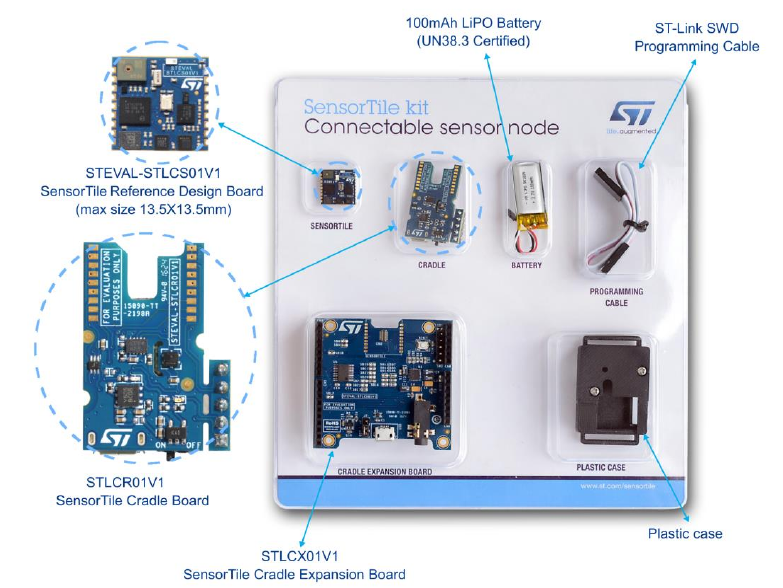
\includegraphics[scale=0.6]{sensortilekit}
\caption{SensorTile Development Kit}
\label{fig:sensortilekit}
\end{center} \end{figure}

\newpage

Figure \ref{fig:sensortile} shows position of main components of the SensorTile board, and Table \ref{table:sensortile} lists their description. \cite{stkitmanual}

\begin{figure}[H] \begin{center}
% \begin{wrapfigure}{l}{0.5\textwidth}
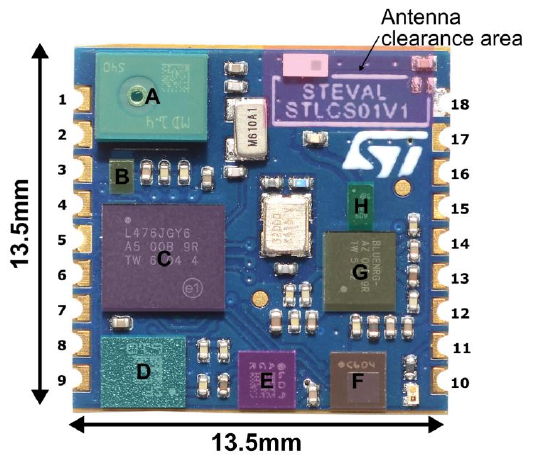
\includegraphics[scale=0.5]{sensortile}
\caption{SensorTile Main Components}
\label{fig:sensortile}
% \end{wrapfigure}
\end{center} \end{figure}

\begin{table}[H]
\centering
\begin{tabular}{@{}|c|l|p{0.55\linewidth}|@{}}
\hline
\toprule
{\bf Reference} & {\bf Device} & {\bf Description} \\ \hline
\midrule
A & MP34DT04      & MEMS audio sensor digital microphone \\ \hline
B & LD39115J18R   & 150 mA low quiescent current low noise LDO 1.8 V \\ \hline
C & STM32L476 MCU & ARM Cortex-M4 32-bit microcontroller \\ \hline
D & LSM6DSM       & iNEMO inertial module: low-power 3D accelerometer and 3D gyroscope \\ \hline
E & LSM303AGR     & Ultra-compact high-performance eCompass module: ultra-low power 3D accelerometer and 3D magnetometer \\ \hline
F & LPS22HB       & MEMS nano pressure sensor: 260-1260 hPa absolute digital output barometer \\ \hline
G & BlueNRG-MS    & Bluetooth low energy network processor \\ \hline
H & BALF-NRG01D3  & 50 Ω balun with integrated harmonic filter \\ \hline
\bottomrule
\end{tabular}
\caption{SensorTile Main Components}
\label{table:sensortile}
\end{table}

\newpage

By default, the SensorTile comes loaded

\newpage
\section{Android App}
\lipsum[1]

\newpage
\section{Analysis \& Results}
\lipsum[1]
